\chapter{Data Manipulation and Its Representation}
\label{sec:datamanip}

In this Chapter a closer look two a couple more of modules is given. These modules result to be very useful in managing financial data and to report results of our analysis.

\section{Getting Data}\label{getting-data}

The first step of any analysis is usually the one that involves selection and manipulation of data we want to process. Data sources can be various (e.g. website, figures, twitter messages, CSV or Excel files\ldots) and partially reflect its nature which can range from \emph{unstructured} data (without any inherent structure, e.g. social media data) to completely \emph{structured} data (where the data model is defined and usually there is no error associated, e.g. stock trading data).
Various modules are available in \texttt{python} in order to gather financial data for our studies: \texttt{quandl}~\cite{bib:quandl}, \texttt{yfinance}~\cite{bib:yfinance},\texttt{ffn}~\cite{bib:ffn}\ldots

Below a simple example using \texttt{yfinance}, that retrieves the closing prices of few securities. The same job with \texttt{quandl} is just a little bit more complicated since it involves the request for a token, but it just takes few minutes more.  

\begin{ipython}
import yfinance as yf

tickers = ['SPY','TLT','MSFT']
	
proxy = yf.Tickers(tickers)

data = proxy.history(start="2021-01-01", end="2021-08-10")
print (data.head())
\end{ipython}
\begin{ioutput}
[*********************100%***********************]  3 of 3 completed
                 Close                         Dividends            \
                  MSFT         SPY         TLT      MSFT  SPY  TLT   
Date                                                                 
2020-12-31  221.397675  371.444244  156.292892       0.0  0.0  0.0   
2021-01-04  216.689423  366.387390  156.104645       0.0  0.0  0.0   
2021-01-05  216.898438  368.910828  154.945297       0.0  0.0  0.0   
2021-01-06  211.274414  371.116394  151.764557       0.0  0.0  0.0   
2021-01-07  217.286652  376.630249  150.426834       0.0  0.0  0.0   

                  High                                 Low  ...              \
                  MSFT         SPY         TLT        MSFT  ...         TLT   
Date                                                        ...               
2020-12-31  221.975010  372.219162  156.639710  218.670263  ...  156.015445   
2021-01-04  221.975014  373.004005  156.738813  213.822655  ...  155.113756   
2021-01-05  217.515598  370.073219  155.520015  214.708553  ...  154.241775   
2021-01-06  215.494931  374.524071  152.448273  210.965841  ...  150.902473   
2021-01-07  218.331828  377.425025  150.783555  212.727716  ...  149.881842   

                  Open                                 Stock Splits    Volume  \
MSFT               SPY         TLT                     MSFT SPY TLT      MSFT   
Date                                                                            
2020-12-31  220.680983  369.357919  156.025363            0   0   0  20942100   
2021-01-04  221.507173  372.864902  155.242576            0   0   0  37130100   
2021-01-05  216.261380  365.701890  155.520015            0   0   0  23823000   
2021-01-06  211.194780  367.301414  152.418547            0   0   0  35930700   
2021-01-07  213.056186  373.649793  150.407012            0   0   0  27694500   


                  SPY       TLT  
Date                             
2020-12-31   78520700   7742100  
2021-01-04  110210800  13152900  
2021-01-05   66426200  10458100  
2021-01-06  107997700  22827300  
2021-01-07   68766800  14651900  

[5 rows x 21 columns]
\end{ioutput}

The \texttt{history} method returns a dataframe (a particular data structure that will be described later in this Chapter) with a lot of information concerning the selected stocks like open and close prices, dividends, volume etc.
Beside the \texttt{start} and \texttt{end} parameters which define the range in which to retrieve data another useful one is \texttt{interval} which specifies its granularity. It can take the following values: 1m, 2m, 5m, 15m, 30m, 60m, 90m, 1h, 1d, 5d, 1wk, 1mo, 3mo. However it is important to note that the 1m data is only retrievable for the last 7 days, and anything intraday (interval <1d) only for the last 60 days.  
In the following example we are going to download the monthly historical series of the closing price of our stocks.

\begin{ipython}
data = proxy.history(start="2021-01-01", end="2021-08-10", interval='1mo')['Close']
print (data.head())
\end{ipython}
\begin{ioutput}
[*********************100%***********************]  3 of 3 completed
                  MSFT         SPY         TLT
Date                                          
2021-01-01  230.893845  367.659088  150.615112
2021-02-01  231.311905  377.882019  141.816010
2021-02-17         NaN         NaN         NaN
2021-03-01  235.226837  393.747986  134.371506
2021-03-19         NaN         NaN         NaN
\end{ioutput}
Note that the table contains also dates in which may be dividends (in this case there are none so the rows are NaN).

When dealing with just one ticker it could be possible to display all the Financial data related to the company by using \texttt{info}. It will show all the information regarding the company including its Sector, No. of Employees, Business Summary, etc.

\begin{ipython}
proxy = yf.Ticker('MSFT')

print (proxy.info)
\end{ipython}
\begin{ioutput}
\{'zip': '98052-6399', 'sector': 'Technology', 'fullTimeEmployees': 181000, 
'longBusinessSummary': 'Microsoft Corporation develops, ...'companyOfficers': [], 
'website': 'http://www.microsoft.com', 'maxAge': 1, 'address1': 'One Microsoft Way', 
'industry': 'Software-Infrastructure', 'ebitdaMargins': 0.48080003, ....\}
\end{ioutput}

Financial Data Analyst requires the details about the Dividends and Splits the company has given to its shareholders. With the \texttt{actions} function, we can download this.

\begin{ipython}
print (proxy.actions)
\end{ipython}
\begin{ioutput}
            Dividends  Stock Splits
Date                               
1987-09-21       0.00           2.0
1990-04-16       0.00           2.0
1991-06-27       0.00           1.5
1992-06-15       0.00           1.5
1994-05-23       0.00           2.0
...               ...           ...
2020-05-20       0.51           0.0
2020-08-19       0.51           0.0
2020-11-18       0.56           0.0
2021-02-17       0.56           0.0
2021-05-19       0.56           0.0

[79 rows x 2 columns]
\end{ioutput}

Other than the \texttt{actions} function we can use \texttt{dividends} and \texttt{splits} functions separately to view them individually.

To know the sustainability of the stock there is a predefined function named \texttt{sustainability} which can be used to display data about the sustainability of the company.

\begin{ipython}
print (proxy.sustainability)
\end{ipython}
\begin{ioutput}
                                     Value
2021-5                                    
palmOil                              False
controversialWeapons                 False
gambling                             False
socialScore                           9.37
nuclear                              False
furLeather                           False
alcoholic                            False
gmo                                  False
catholic                             False
socialPercentile                      None
peerCount                              103
governanceScore                       4.83
environmentPercentile                 None
animalTesting                        False
tobacco                              False
totalEsg                             14.63
highestControversy                       3
esgPerformance                  UNDER_PERF
coal                                 False
pesticides                           False
adult                                False
percentile                            7.59
peerGroup              Software & Services
smallArms                            False
environmentScore                      0.42
governancePercentile                  None
militaryContract                     False
\end{ioutput}

Recommendations for buying or selling a company’s stock is provided by different Finacial Firms. In order to analyze the stock price, we must know what these firms recommend. To analyze the recommendations we can use the \texttt{recommendations} function.

\begin{ipython}
print (proxy.recommendations)
\end{ipython}
\begin{ioutput}
                               Firm       To Grade From Grade Action
Date                                                                
2012-03-16 08:19:00  Argus Research            Buy                up
2012-03-19 14:00:00  Hilliard Lyons  Long-Term Buy              main
2012-03-22 07:03:00  Morgan Stanley     Overweight              main
2012-04-03 11:53:00             UBS            Buy              main
2012-04-20 06:18:00   Deutsche Bank            Buy              main
...                             ...            ...        ...    ...
2021-07-28 14:47:46        Barclays     Overweight              main
2021-07-28 14:49:16       Citigroup            Buy              main
2021-07-28 14:51:12          Mizuho            Buy              main
2021-07-28 14:54:54   Credit Suisse     Outperform              main
2021-07-29 10:53:54       JP Morgan     Overweight              main
\end{ioutput}

\texttt{calendar} function can be used to know about the earnings and revenue of the company.

\begin{ipython}
print (proxy.calendar)
\end{ipython}
\begin{ioutput}
                                    0                    1
Earnings Date     2021-10-25 10:59:00  2021-10-29 12:00:00
Earnings Average                 1.90                 1.90
Earnings Low                     1.64                 1.64
Earnings High                    2.03                 2.03
Revenue Average           44102900000          44102900000
Revenue Low               40850000000          40850000000
Revenue High              44914700000          44914700000
\end{ioutput}

For every company listed on the stock market, there is a unique ISIN (International Securities Identification Number) no. we can retrieve this number using \texttt{isin} function

\begin{ipython}
print (proxy.isin)
\end{ipython}
\begin{ioutput}
US5949181045
\end{ioutput}

During option trading we must know about the option expiry date, using the \texttt{options} function we can retrieve the Option Expiry Date of that particular stock.

\begin{ipython}
print (proxy.options)
\end{ipython}
\begin{ioutput}
('2021-08-13', '2021-08-20', '2021-08-27', '2021-09-03', '2021-09-10', 
 '2021-09-17', '2021-09-24', '2021-10-15', '2021-11-19', '2021-12-17', 
 '2022-01-21', '2022-03-18', '2022-06-17', '2022-09-16', '2023-01-20', 
 '2023-03-17', '2023-06-16')
\end{ioutput}

Finally to get for example calls data:
\begin{ipython}
opt = proxy.option_chain(date='2021-08-13')
print (opt.calls)
\end{ipython}
\begin{ioutput}
         contractSymbol       lastTradeDate  strike  lastPrice  bid  ask  \
0   MSFT210813C00180000 2021-08-09 14:48:40   180.0     109.05  0.0  0.0   
1   MSFT210813C00185000 2021-08-09 13:35:15   185.0     105.45  0.0  0.0   
2   MSFT210813C00190000 2021-08-03 15:04:10   190.0      95.10  0.0  0.0   
3   MSFT210813C00195000 2021-08-03 14:35:40   195.0      89.60  0.0  0.0   
4   MSFT210813C00200000 2021-08-09 13:37:35   200.0      89.26  0.0  0.0   
5   MSFT210813C00205000 2021-08-03 14:11:33   205.0      79.85  0.0  0.0   
...

    change  percentChange   volume  openInterest  impliedVolatility  \
0      0.0            0.0      5.0             5           0.000010   
1      0.0            0.0      3.0             0           0.000010   
2      0.0            0.0      NaN             4           0.000010   
3      0.0            0.0      1.0            10           0.000010   
4      0.0            0.0      1.0             8           0.000010   
5      0.0            0.0      1.0             0           0.000010   
...

    inTheMoney contractSize currency  
0         True      REGULAR      USD  
1         True      REGULAR      USD  
2         True      REGULAR      USD  
3         True      REGULAR      USD  
4         True      REGULAR      USD  
5         True      REGULAR      USD  
\end{ioutput}

These are the main functions of \texttt{yfinance} which can be used for stock data analysis. A more detailed guide can be found \href{https://algotrading101.com/learn/yfinance-guide/}{\emph{here}}.

\section{Manipulating Data}
Our primary goal, before start processing data, is to collect and store the information in a suitable data structure. \texttt{python} provides a very useful module, called \texttt{pandas}, which allows to collect and save data in \emph{dataframe} objects that can be later on manipulated for analysis purposes~\cite{pandas}.

Looking at \texttt{pandas} manual, dataframes are defined as multi-dimensional, size-mutable, potentially heterogeneous, tabular data structure with labeled axes (rows and columns), in much simpler words it is a table whose structure can be modified.
It contains multiple methods for convenient data filtering and in addition has a lot of utilities to load and 
save data pretty easily.

Dataframes can be created by:
\begin{itemize}
	\tightlist
\item importing data from file (\href{https://github.com/matteosan1/finance_course/blob/develop/libro/input_files/sample.xlsx?raw=true}{sample.xlsx}, \href{https://raw.githubusercontent.com/matteosan1/finance_course/develop/libro/input_files/sample.csv}{sample.csv});
\item creating by hand data and then filling the dataframe.
\end{itemize}

\begin{ipython}
import pandas as pd

# reading from file
df1 = pd.read_excel('sample.xlsx') # Excel file
df2 = pd.read_csv('sample.csv') # Comma Separated file
print (df1.head(11)) # show just few rows at the beginning
\end{ipython}
\begin{ioutput}
         Date      Price     Volume
0  2020-05-18  78.739998  135178400
1  2020-05-19  78.285004  101729600
2  2020-05-20  79.807503  111504800
3  2020-05-21  79.212502  102688800
4  2020-05-22  79.722504   81803200
5  2020-05-26  79.182503  125522000
6  2020-05-27  79.527496  112945200
7  2020-05-28  79.562500  133560800
8  2020-05-29  79.485001  153532400
9  2020-06-01  80.462502   80791200
10 2020-06-02  80.834999   87642800
\end{ioutput}

\begin{ipython}
# creating some data in a dictionary
d = {"Name":["Elisa", "Roberto", "Ciccio", "Topolino", "Gigi"],
	 "Age":[1, 27, 25, 24, 31],
	 "Points":[100, 120, 95, 1300, 101]}

# filling the dataframe
df = pd.DataFrame(d)
print (df.head())
\end{ipython}
\begin{ioutput}
       Name  Age     Points
0     Elisa    1        100
1   Roberto   27        120
2    Ciccio   25         95
3  Topolino   24       1300
4      Gigi   31        101
\end{ioutput}

Of course with \texttt{pandas} it is possible to perform a large number of operations on dataframes. 
For example it is possible to add a column as a result of an operation on other columns. 
Looking back at dataframe \texttt{df1} it is possible to add a column with the daily variation of the price.

\begin{ipython}
import numpy as np

# first let's add an empty column
df1['Variation'] = np.nan # nan stands for not a number

# loop on the Price column, compute the variation and fill the column
# len returns the number of rows of a dataframe
for i in range(1, len(df1)):
    # select the ith row and fill "Variation"
    # loc takes as inputs row and colum-name
    df1.loc[i, "Variation"] = (df1.loc[i, "Price"] - df1.loc[i-1, "Price"]) /
        df1.loc[i-1, "Price"]
print (df1.head())
\end{ipython}
\begin{ioutput}
        Date      Price     Volume  Variation
0 2020-05-18  78.739998  135178400        NaN
1 2020-05-19  78.285004  101729600  -0.005778
2 2020-05-20  79.807503  111504800   0.019448
3 2020-05-21  79.212502  102688800  -0.007455
4 2020-05-22  79.722504   81803200   0.006438	
\end{ioutput}
\noindent
Of course the first ``variation'' value is NaN since there is no previous price to compare with. NaN, short for \emph{not a number}, represents the \texttt{null} value, it is the value that is given to missing fields in a row. 

\subsection{Manage Data}\label{manage-data}

Once we have created our dataframe we may want to preliminary process data to perform very common operations like:

\begin{itemize}
	\tightlist
\item remove unwanted observations or outliers;
\item handle missing data;
\item filter, sort and clean data.
\end{itemize}

\subsection{Unwanted observations and outliers}

\subsubsection{Duplicates}

It may happen that our data has duplicates (e.g. those can arise when combining two datasets), or the dataset contains irrelevant fields for the specific study we are carrying on. To find and remove duplicates \texttt{pandas} has convenient methods:

\begin{ipython}
# find duplicates based on all columns
# and show just the first 15 results
#print (df1.duplicated()[:15])

# find duplicates based on'Price'
# and show just the first 15 results
print (df1.duplicated(subset=['Price'])[:15] )
\end{ipython}
\begin{ioutput}
0     False
1     False
2     False
3     False
4      True
5     False
6     False
7     False
8     False
9     False
10    False
11     True
12     True
13    False
14    False
dtype: bool
\end{ioutput}

\begin{ipython}
print ("Initial number of rows: {}".format(len(df1)))

# remove duplicates
# where the second argument can be `first` , `last`
# or `False` (consider all of the same values as duplicates).

df1 = df1.drop_duplicates(subset='Price', keep='first')
print ("Number of columns after drop: {}".format(len(df1)))
\end{ipython}
\begin{ioutput}
Initial number of rows: 254
Number of columns after drop: 248
\end{ioutput}

If we would like to drop irrelevant columns for our analysis it is enough to:

\begin{ipython}
df2 = df2.drop(columns=['Volume'])
print (df2.head())
\end{ipython}
\begin{ioutput}
         Date      Price
0  18/05/2020  78.739998
1  19/05/2020  78.285004
2  20/05/2020  79.807503
3  21/05/2020  79.212502
4  22/05/2020  79.722504
\end{ioutput}
        
If instead we just want to remove few rows we can select them by index:

\begin{ipython}
# we remove row 0th and 2nd
# axis=0 means use the index column
df2 = df2.drop([0, 2], axis=0)
print (df2.head())
\end{ipython}
\begin{ioutput}
         Date      Price
1  19/05/2020  78.285004
3  21/05/2020  79.212502
4  22/05/2020  79.722504
5  26/05/2020  79.182503
6  27/05/2020  79.527496
\end{ioutput}
        
Changing the column that act as index we can select the rows also by other attributes:

\begin{ipython}
# tell pandas to use Date as index column
df2 = df2.set_index('Date')

# select row to remove by date at this point
df2 = df2.drop(["2000-07-31"], axis=0)
print (df2.head())
\end{ipython}
\begin{ioutput}
                Price
Date                 
21/05/2020  79.212502
22/05/2020  79.722504
26/05/2020  79.182503
27/05/2020  79.527496
28/05/2020  79.562500
\end{ioutput}
        
\subsubsection{Outliers}\label{outliers}

An outlier is an observation that lies outside the overall pattern of a distribution. Common causes can be human, measurement or experimental errors. Outliers must be handled carefully and should be removed cautiously, \emph{outliers are innocent until proven guilty}. We may have removed the most interesting part of our dataset !

The core statistics about a particular column can be studied by the \texttt{describe()} method which returns the following information:
\begin{itemize}
	\tightlist
\item for numeric columns: the value count, mean, standard deviation, minimum, maximum and 25th, 50th and 75h quantiles for the data in a column;
\item for string columns: the number of unique entries, the most frequent occurring value (\emph{top}), and the number of times the top value occurs (\emph{freq}).
\end{itemize}

\begin{ipython}
print (df1.describe())
\end{ipython}
\begin{ioutput}
              Price        Volume   Variation
count    248.000000  2.430000e+02  247.000000
mean     163.747117  1.287922e+08    0.393586
std      748.572478  5.309638e+07    6.210597
min       78.285004  4.669130e+07   -0.990255
25%      110.274997  9.032360e+07   -0.008365
50%      120.109996  1.129452e+08    0.001749
75%      128.132504  1.536495e+08    0.016365
max    11902.000000  3.743368e+08   97.599951
\end{ioutput}
        
Looking at mean and std and comparing it with min and max values we could find a range outside of which we may have outliers. For example 11902.0 is several standard deviation away the mean which may indicate that it is not a good value.

Another way to spot outliers is to plot column distributions and again \texttt{pandas} comes to help us:
\begin{ipython}
df1.hist("Variation", bins=np.arange(0, 100, 1))
\end{ipython}

\begin{figure}
	\centering
	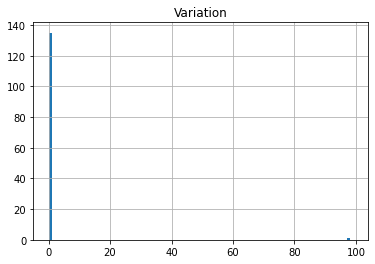
\includegraphics[width=0.7\linewidth]{figures/volume_plot}
\end{figure}

From the histograms it is clear how the value of 97.60, is far from general population. This doesn't mean it is necessarily wrong but it should make ring a bell in our head\ldots

To remove outliers from data we can either remove the entire rows or replace the suspicious values by a default one 
(e.g. 0, 1, a threshold value\ldots).

\textbf{Note}: missing data may be informative itself~!~When filling the gap with \emph{artificial data} (e.g. mean, median, std\ldots) having similar properties than real observation, the added value won't be scientifically valid, no matter how sophisticated your filling method is.

\begin{ipython}
import numpy as np

df2 = df2.replace(11902, 500) # replace 11902 with 500
df2 = df2.replace(11902, np.nan) # replace 11902 with NaN
df2 = df2.mask(df1 >= 150, 5) # replace every element >=600 with 5
\end{ipython}

\subsection{Handle Missing Data}\label{handle-missing-data}

Usually when importing data with \texttt{pandas} we may have some NaN values. Like for the outliers we can use the \texttt{replace} or \texttt{mask} methods to remove the NaNs. In case the whole row as NaN it may be wise to drop it entirely.

Additionally we can use \texttt{dropna()} which remove all the NaN in the dataframe at once.

\begin{ipython}
df1 = df1.dropna()
print ("Number of rows after dropping NaN: {}".format(len(df1)))
\end{ipython}
\begin{ioutput}
Number of rows after dropping NaN: 242
\end{ioutput}

\subsection{Filter, Sort and Clean Data}\label{filter-sort-and-clean-data}

\subsubsection{Filtering}\label{filtering}

When we work with huge datasets we may reach computational limits (e.g. insufficient memory, CPU performance, too slow processing time\ldots) and in those cases it can be helpful to filter data by attributes for example by splitting by time or some other property.

Assuming to have the following table and putting back the volume column

\begin{ipython}
# df.iloc[row, col]
# NOTE: iloc takes row and column index (two numbers)
# loc instead takes row index and column name

print (df1.iloc[1, 2]) # returns 62 the volume associated with the row
\end{ipython}
\begin{ioutput}
111504800.0
\end{ioutput}

\begin{ipython}
#df.iloc[row1:row2, col1:col2]
# this is called slicing, remember ?

print (df1.iloc[0:2, 2:3]) # returns rows 0 and 1 of column 2
\end{ipython}
\begin{ioutput}
        Volume
1  101729600.0
2  111504800.0
\end{ioutput}

\begin{ipython}
subset = df1.iloc[:, 1] # select column 1
subset = df1.iloc[2, :] # select row 2
subset = df1.iloc[0:2, :] # select 2 rows
subset = df1.iloc[:2, :] # this is equivalent to before
\end{ipython}

A more advanced way of filtering is the following (it apply a selection on the values). The notation is a bit awkward but very useful:

\begin{ipython}
import datetime

# colon means all the rows
subset = df1[df1.iloc[:, 0] < datetime.datetime(2020, 8, 15)]
print (subset)
\end{ipython}
\begin{ioutput}
         Date       Price       Volume  Variation
1  2020-05-19   78.285004  101729600.0  -0.005778
2  2020-05-20   79.807503  111504800.0   0.019448
3  2020-05-21   79.212502  102688800.0  -0.007455
5  2020-05-22   79.722504   81803200.0   0.006438
6  2020-05-26   79.182503  125522000.0  -0.006774
..        ...         ...          ...        ...
61 2020-08-10  112.727501  212403600.0   0.014535
62 2020-08-11  109.375000  187902400.0  -0.029740
63 2020-08-12  113.010002  165598000.0   0.033234
64 2020-08-13  115.010002  210082000.0   0.017698
65 2020-08-14  114.907501  165565200.0  -0.000891

[61 rows x 4 columns]
\end{ioutput}

\subsubsection{Sorting}\label{sorting}

To sort our data we can use \texttt{sort\_values()} method (it can be specified ascending, descending).

\begin{ipython}
# sort by price then by date in descending order
print (df2.sort_values(by=['Price', "Date"], ascending=False)[:10])
\end{ipython}
\begin{ioutput}
                 Price
Date                  
26/01/2021  143.160004
25/01/2021  142.919998
27/01/2021  142.059998
22/01/2021  139.070007
04/02/2021  137.389999
28/01/2021  137.089996
08/02/2021  136.910004
21/01/2021  136.869995
05/02/2021  136.759995
28/12/2020  136.690002
\end{ioutput}
        
\subsubsection{Cleaning or Regularizing}\label{cleaning-or-regularizing}

As we will see when dealing with machine learning, often we need to regularize our data to improve the stability of a training. One typical situation is when we want to \emph{normalize} data, which means re-scale the values into a range of $[0, 1]$.

\begin{equation*}
\begin{gathered}
x = [1,43,65,23,4,57,87,45,45,23]\\
x_{new} = \cfrac{x - x_{min}}{x_{max} - x_{min}}\\
x_{new} = [0,0.48,0.74,0.25,0.03,0.65,1,0.51,0.51,0.25]
\end{gathered}
\end{equation*}

To apply such a transformation with \texttt{pandas} is very easy since applying the formula to a dataframe implies it is done to each row:

\begin{ipython}
df1['Price'] = (df1['Price'] - df1['Price'].min()) \
    / (df1['Price'].max() - df1['Price'].min())
print (df1.head())
\end{ipython}
\begin{ioutput}
        Date     Price       Volume  Variation
1 2020-05-19  0.000000  101729600.0  -0.005778
2 2020-05-20  0.000129  111504800.0   0.019448
3 2020-05-21  0.000078  102688800.0  -0.007455
5 2020-05-22  0.000122   81803200.0   0.006438
6 2020-05-26  0.000076  125522000.0  -0.006774
\end{ioutput}
        
Another quite common transformation is called \emph{standardization}, essentially we re-scale data to have 0 mean and standard deviation of 1:

\begin{equation}
x_{new} = \cfrac{x-\mu}{\sigma}
\label{eq:standardization}
\end{equation}

Again it is straightforward to do it in \texttt{pandas}:

\begin{ipython}
df1.hist('Volume', bins=np.arange(180, 220, 1))

print (df1['Volume'].mean())
print (df1['Volume'].std())
\end{ipython}
\begin{ioutput}
128765806.61157025
53204829.93713034
\end{ioutput}

\begin{ipython}
df1['Volume'] = (df1['Volume'] - df1['Volume'].mean()) / df1['Volume'].std()
df1.hist('Volume', bins=np.arange(-5, 5, 0.1))

print (df1['Volume'].mean())
print (df1['Volume'].std())
\end{ipython}
\begin{ioutput}
-1.5598174726138563e-17
1.0
\end{ioutput}

Figure~\ref{fig:standardization} shows the comparison of the "volume" distribution before and after stadardization.

\begin{figure}[htb]
	\centering
	\subfloat[Original.]{%
		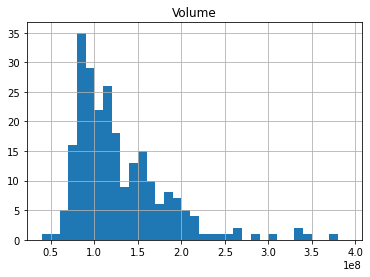
\includegraphics[width=0.45\textwidth]{figures/volume_plot_2}
	}
	\subfloat[Standardized according to Eq.~\ref{eq:standardization}.]{%
		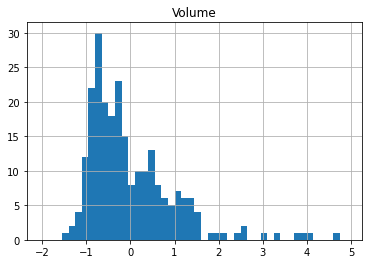
\includegraphics[width=0.45\textwidth]{figures/volume_plot_3}
	}
	\caption{Comparison between "volume" distributions.}
	\label{fig:standardization}
\end{figure}

\subsection{Operations on Data}
Using \texttt{pandas} all sorts of calculations between rows or columns can be made. Some example of that will be shown in the next Chapters, here just a simple application of Moving Average (MA) is described.

In finance, technical analysis is an analysis methodology for forecasting the direction of prices through the study of past market data, primarily price and volume. Technical analysts rely on a combination of technical indicators to study a stock and give insight about possible trading strategies. 

Consider for example a particular indicator called \emph{Bollinger Bands}. It is usually used to provide potential buy / sell signals and to define the prevailing high and low prices in a market to characterize the trading band of a financial instrument or commodity. You can think of Bollinger Bands as a volatility indicator. Bands consist of Moving Average lines, a upper band and lower band. The upper and lower bands are simply MA adding and subtracting standard deviation ($\sigma$), which is a sort of  measurement of volatility. 
\[
\begin{split}
\textrm{Upper Band} & = (\textrm{MA} + K\sigma)\\
\textrm{Lower Band} & = (\textrm{MA} − K\sigma)
\end{split}
\]

In the following example we are going to use a 20 day moving average and $K=2$. Imagine to have the historical series of AMZN stock closing prices. Bollinger Bands can be quickly and easily constructed as follows 

\begin{ipython}
import yfinance as yf
import pandas as pd
import matplotlib.pyplot as plt

proxy = yf.Ticker('AMZN')
df = proxy.history(start='2017-04-02', end='2018-05-02')['Close']

# calculate Moving Average with 20 days window
ma = df.rolling(window=20).mean()

# calculate the standard deviation
rstd = df.rolling(window=20).std()

df['upper'] = ma + 2 * rstd
df['lower'] = ma - 2 * rstd

ax = df.plot(title='AMZN Price and Bollinger Bands', figsize=(10,8))
ax.fill_between(df.index, df['lower'], df['upper'], color='#ADCCFF', alpha='0.4')
ax.set_xlabel('date')
ax.set_ylabel('Price Moving Average')
ax.set_xlim('2017-05-02', '2018-05-02')
ax.grid()
\end{ipython}

The resulting plot is shown in Fig.~\ref{fig:bollinger_bands} which can be interpreted by saying that approximately 90\% of prices lay between the two bands. Therefore the bands can be used to identify potential overbought or oversold conditions. If stock price breaks out the upper band, it could be an overbought condition (indication of short). Similarly, when it breaks out the lower band, it could be oversold condition (indication of long). 

\begin{figure}[htb]
	\centering
	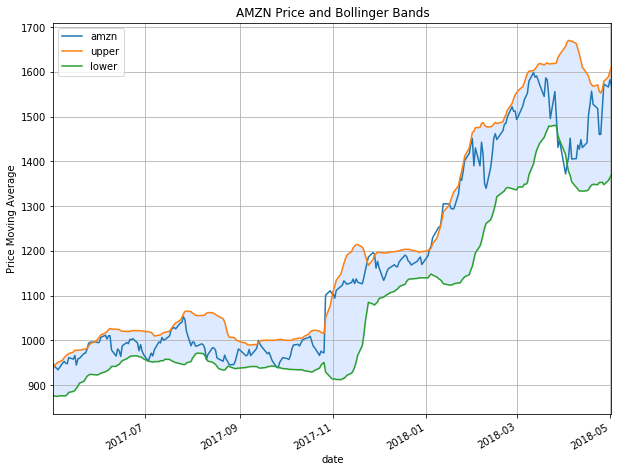
\includegraphics[width=0.7\textwidth]{figures/bollinger_bands}
	\caption{Bollinger Bands plot applied to AMZN historical prices.}
	\label{fig:bollinger_bands}
\end{figure}

\section{Plotting in \texttt{python}}\label{plotting-in-python}

As we have just seen \texttt{pandas} allows to quickly draw histograms of dataframe columns, but during an analysis we may want to plot distributions from \texttt{list} or objects not stored in a dataframe. Furthermore the simple although very useful interface doesn't grant full access to all plotting features that we need to produce nice and informative plots.

In order to do so we can use the \texttt{matplotlib} module which is specifically dedicated to plotting (\texttt{pandas} interface is based on the same module indeed). 

In the next Sections we will look briefly to its capabilities. For those interested a more detailed and comprehensive documentation can be found at~\cite{matplotlib}.

\subsection{Canvas}\label{canvas}

The first element we need to plot is a \emph{canvas}, the white rectangular space where we draw our data. \texttt{Matplotlib} provides a default canvas if no specific command is given (a 640x480 pixels space) but you can customize it by specifying many different parameters, the most commonly are:

\begin{itemize}
	\tightlist
	\item
	\texttt{figsize}: width, height in inches. If not provided, defaults
	to \([6.4, 4.8]\);
	\item
	\texttt{dpi}: resolution of the figure. If not provided, defaults to
	100;
	\item
	\texttt{facecolor}: the background color. If not provided, defaults to
	\texttt{'white'}, or \texttt{'w'}.
\end{itemize}

In the following example we create a canvas (8 inches x 5 inches) with a resolution of 80 dots per inches (dpi) and a green background color.

\begin{ipython}
from matplotlib import pyplot as plt

fig = plt.figure(figsize=(8,5), dpi=80, facecolor='green')
\end{ipython}

Once we have a canvas we cannot even draw it unless we have some plot to
show. So let's see the most commonly used types of plot.

\subsection{Chart Object}\label{chart-object}

Below a concise list of the main chart objects that are used when presenting financial data.

\subsubsection{Histograms}\label{histograms}

A histogram is an approximate representation of the distribution of numerical data. To construct a histogram, the first step is to \emph{bin} (or \emph{bucket}) the range of values (i.e. divide the entire range of values into a series of intervals) and then count how many values fall into each interval.

If the bins are of equal size, a rectangle is erected over the bin with height proportional to the frequency (i.e. the number of cases in each bin).

However, bins need not be of equal width; in that case, the erected rectangle is defined to have its area proportional to the frequency of cases in the bin. The vertical axis is then not the frequency but frequency density (i.e. the number of cases per unit of the variable on the horizontal axis).

To create an histogram with \texttt{matplotlib} it is enough to pass a list (or a \texttt{numpy.array}) with data to represent to the function \texttt{hist} and then call \texttt{show()} to actually draw the plot (I have also used the previously defined canvas just to show the results), Fig.~\ref{fig:histo1}.

\begin{ipython}
y1 = [40.9, 47.7, 40.6, 43.0, 45.4, 42.3, 33.8, 49.6,
47.6, 52.3, 43.1, 36.5, 43.7, 52.4, 37.0, 42.4, 38.4, 39.9, 40.6, 35.7, 42.4,
38.3, 43.6, 38.5, 43.5, 42.9, 42.1, 39.8, 35.8, 44.1,
41.5, 42.6, 45.4, 38.6, 37.3, 37.8, 48.1, 44.8, 32.7, 40.3]

fig = plt.figure(figsize=(8,5), dpi=80, facecolor='green')
plt.hist(y1)
plt.show()
\end{ipython}

\begin{figure}[htb]
	\centering
	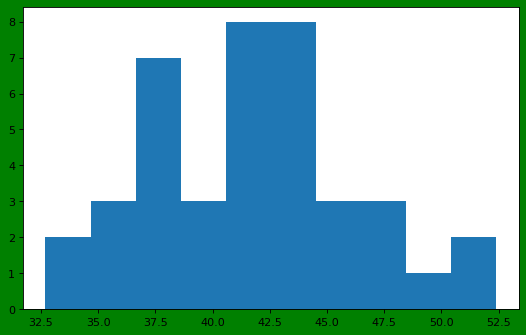
\includegraphics[width=0.7\textwidth]{figures/histo1}
	\caption{Example of histogram drawn on the previously defined canvas.}
	\label{fig:histo1}
\end{figure}

If you are not satisfied with the default binning and/or you want to
change the range shown in the plot, those can be specified in the call
to \texttt{hist} like this (see Fig.~\ref{fig:histo2})

\begin{ipython}
# after data there is the number of equally spaced bins
# to be used, then the range

plt.hist(y, 50, range=(30, 50))
plt.show()
\end{ipython}

\begin{figure}[htb]
	\centering
	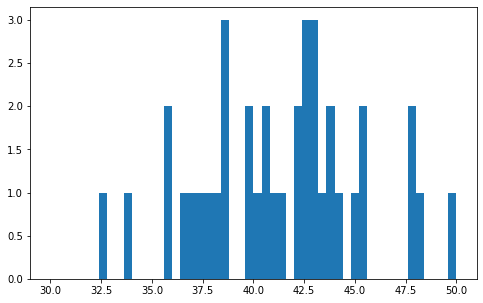
\includegraphics[width=0.7\textwidth]{figures/histo2}
	\caption{Example of histogram with custom binning and range.}
	\label{fig:histo2}
\end{figure}

Passing other parameters it is possible to modify the style of the
histogram, like its color which can be specified by name. For
the basic built-in colors, you can also use a single letter

\begin{itemize}
	\tightlist
	\item
	b: blue
	\item
	g: green
	\item
	r: red
	\item
	c: cyan
	\item
	m: magenta
	\item
	y: yellow
	\item
	k: black
	\item
	w: white
\end{itemize}

Plotting multiple histograms on the same canvas is as easy as calling
various times \texttt{hist} (binning should be the same for each
histogram).

To each object that is plotted can be associated a label, passing the
corresponding parameter to the object call, so that we can build a
legend. Latex symbols can be used whenever text is used, the characters
have to enclosed between dollar symbols (i.e. \$\\mu\$). Legend that
will be shown on the canvas with the command \texttt{legend()}.
A grid can be added to the plot with \texttt{plt.grid(True)} for a nicer
look. Figure~\ref{fig:histo3} shows such an example.

\begin{ipython}
y2 = [40.6, 40.5, 37.3, 37.6, 39.0, 38.5, 36.0, 
      39.0, 36.8, 41.4, 41.9, 39.9, 39.0, 37.7, 
      35.0, 37.9, 35.2, 39.5, 37.7, 38.4, 42.4, 
      38.1, 39.0, 34.7, 37.1, 36.6, 37.0, 40.8, 
      39.0, 41.5]

plt.hist(y1, 50, range=(30, 50), color='red', label='Red Hist')
plt.hist(y2, 50, range=(30, 50), color='yellow', label='Yellow Hist')
plt.legend()
plt.grid(True)
plt.show()
\end{ipython}

\begin{figure}[htb]
	\centering
	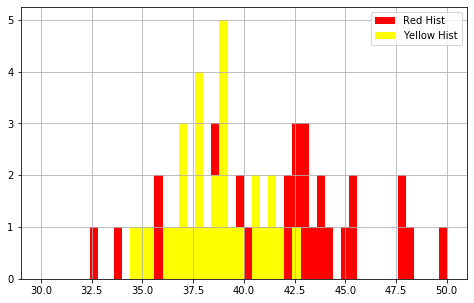
\includegraphics[width=0.7\textwidth]{figures/histo3}
	\caption{Plotting two histograms on the same canvas with different colors and the 
		corresponding legend.}
	\label{fig:histo3}
\end{figure}

\subsubsection{Scatter Plot}\label{scatter}

A scatter plot is a type of plot using Cartesian coordinates to display values of two variables for a set of data. If the points are coded (color/shape/size), one additional variable can be displayed.

The data are displayed as a collection of points, each having the value of one variable determining the position on the horizontal axis and the value of the other variable determining the position on the vertical axis.

To create such an object it is enough to call \texttt{scatter} and pass the \(x\) and \(y\) lists, Fig.~\ref{fig:scatter1}.

\begin{ipython}
y1 = [26.2, 5.4, 7.7, 3.8, 24.7, -5.5, 36.4, 12.9, 25.2, 21.0, 39.6,
      5.9, 24.8, 25.7, 42.3, 21.5, 32.3, 26.7, 37.4, 44.3, 29.0,
      52.9, 52.0, 49.5, 55.0, 40.7, 47.8, 41.1, 49.3, 58.8, 48.1,
      52.5, 51.1, 51.0, 54.3, 62.4, 52.8, 67.8, 83.6, 75.9]

x = range(len(y1))
plt.scatter(x, y1)
plt.show()
\end{ipython}

\begin{figure}[htb]
	\centering
	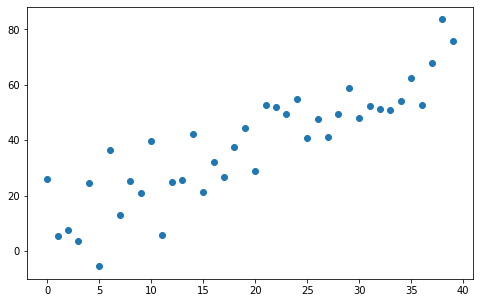
\includegraphics[width=0.7\textwidth]{figures/scatter}
	\caption{Example of scatter plot.}
	\label{fig:scatter}
\end{figure}

Other parameters can be passed to \texttt{scatter} the most useful are

\begin{itemize}
	\tightlist
	\item
	\texttt{label}: label the scatter plot for the legend;
	\item
	\texttt{color}: set the color of the marker;
	\item
	\texttt{marker}: set the style of the marker defined with a single
	character (+,*, o, x\ldots{});
	\item
	\texttt{s=}: set the size of the marker.
\end{itemize}

And of course multiple scatter plot can be shown together in the same
canvas calling \texttt{scatter} accordingly (see Fig.~\ref{fig:scatter2}).

\begin{ipython}
y2 = [22.2, 3.4, 7.7, 5.8, 28.7, 0.5, 44.4, 22.9, 37.2, 35.0, 55.6,
      23.9, 44.8, 47.7, 66.3, 47.5, 60.3, 56.7, 69.4, 78.3, 65.0,
      90.9, 92.0, 91.5, 99.0, 86.7, 95.8, 91.1, 101.3, 112.8,
      104.1, 110.5, 111.1, 113.0, 118.3, 128.4, 120.8, 137.8, 155.6, 149.9]

plt.scatter(range(len(y1)), y1, s=10, marker="o",
color="lightblue", label="1st Scatter")
plt.scatter(range(len(y2)), y2, s=30, marker="*",
color="brown", label="2nd Scatter")
plt.legend()
plt.show()
\end{ipython}

\begin{figure}[htb]
	\centering
	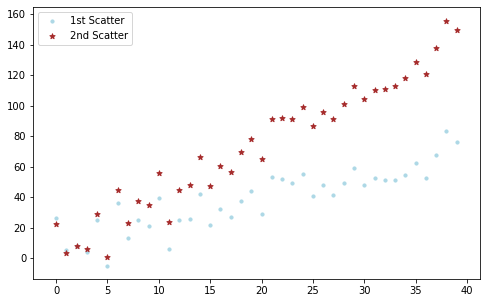
\includegraphics[width=0.65\textwidth]{figures/scatter2}
	\caption{More advanced scatter plot example.}
	\label{fig:scatter2}
\end{figure}

\subsubsection{Plot}\label{plot}

If you want to still plot \(x\) and \(y\) points but they should be
connected with a line you can use the function \texttt{plot}. It acts
similarly to \texttt{scatter} but the graphical result will be
different.

For example below the same two scatter plots of the previous example are
plotted with \texttt{plot}, Figure~\ref{fig:plot1}

\begin{ipython}
plt.plot(x, y1, label="1st Plot")
plt.plot(x, y2, label="2nd Plot")
plt.legend()
plt.show()
\end{ipython}

\begin{figure}[htb]
	\centering
	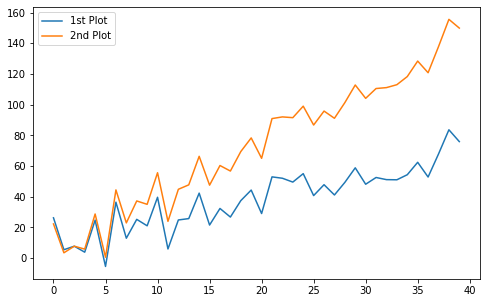
\includegraphics[width=0.65\textwidth]{figures/plot1}
	\caption{Example of scatter plot where points are connected by a line.}
	\label{fig:plot1}
\end{figure}

In this case the parameters the parameters allow to control the line
style and the possibility to add the marker at each point (see Fig.~\ref{fig:plot2})

\begin{itemize}
	\tightlist
	\item
	\texttt{label}: label the scatter plot fot the legend;
	\item
	\texttt{color}: set the color of the marker and the line;
	\item
	\texttt{marker}: set the sityle of the marker defined with a single
	character (+,*, o, x\ldots{});
	\item
	\texttt{s}: set the size of the marker;
	\item
	\texttt{linestyle}: style of the line (`-', `--', `-.', `:');
	\item
	\texttt{linewidth}: thickness of the line.
\end{itemize}

\begin{ipython}
plt.plot(x, y1, marker="+", linestyle=":", color="darkgreen", label="1st Plot")
plt.plot(x, y2, marker="x", linewidth=5, color="pink", label="2nd Plot")
plt.legend()
plt.show()
\end{ipython}

\begin{figure}[htb]
	\centering
	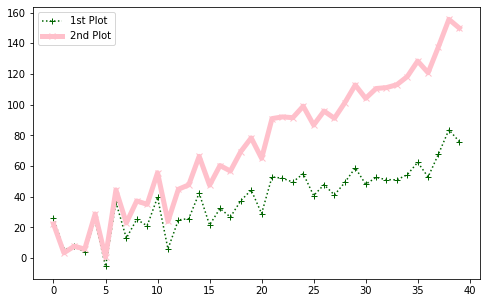
\includegraphics[width=0.7\textwidth]{figures/plot2}
	\caption{More refined example of connected scatter plot.}
	\label{fig:plot2}
\end{figure}

\subsubsection{Plotting a Function}\label{plotting-a-function}

Functions can be plotted using the \texttt{plot} method as well. They can be
functions from \texttt{python} modules or user-defined.

As an example let's try to plot \(\mathrm{sin}(x/2)\), in the example we
will use \texttt{numpy.arange} function which extends the functionalities
of the standard \texttt{range} allowing for non integer parameters.

In such cases it is always recommended to use \texttt{numpy} functions
and not those defined in \texttt{math} since they also accept arrays in
input for a faster processing (i.e. it is not need to loop over each
\(x\) to compute the function values since it is done automatically).
Figure~\ref{fig:sinx_x} reports the result of the code below.

\begin{ipython}
from numpy import arange, sin

def func(x):
    return sin(x/2)
xs = arange(-10, 10, 0.01)

fig = plt.figure(figsize=(8,5))
plt.plot(xs, func(xs))
plt.show()
\end{ipython}

\begin{figure}[htb]
	\centering
	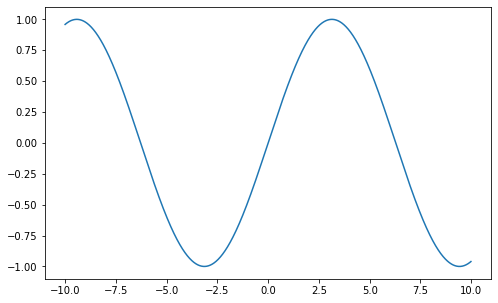
\includegraphics[width=0.65\textwidth]{figures/sinx_x}
	\caption{Example of a plot of a function, in this case \(\mathrm{sin}(x/2)\).}
	\label{fig:sinx_x}
\end{figure}

\subsection{Axes}\label{axes}

The axis of a any plot can be formatted with many options.

First of all the axis range can be controlled with
\texttt{xlim(min, max} and \texttt{ylim(min, max}. Then labels can be
added with \texttt{xlabel(myLabel)} and \texttt{ylabel(myLabel)}. A
global title to the plot can also be specified with
\texttt{plt.title(myTitle)}.

Referring to the previous example we can write

\begin{ipython}
fig = plt.figure(figsize=(8,5))
plt.plot(x, y1, marker="+", linestyle=":", color="darkgreen", label="1st Plot")
plt.plot(x, y2, marker="x", linewidth=5, color="pink", label="2nd Plot")
plt.title("Plot Title")
plt.xlabel("x label")
plt.ylabel("y label")
plt.legend()
plt.show()
\end{ipython}
\noindent
and see the result in Fig.~\ref{fig:axis1}.

\begin{figure}[htb]
	\centering
	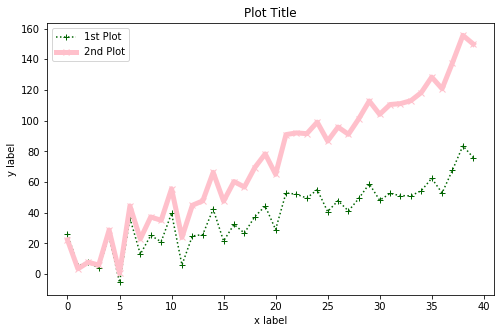
\includegraphics[width=0.65\textwidth]{figures/axis1}
	\caption{Improving the look of a plot by formatting the axis.}
	\label{fig:axis1}
\end{figure}

It can also be specified if axis has to be in linear or log scale with
\texttt{xscale("log")} and/or \texttt{yscale("log")}, see Fig.~\ref{fig:axis2}.

\begin{ipython}
fig = plt.figure(figsize=(8,5))
plt.plot(x, y1, marker="+", linestyle=":", color="darkgreen", label="1st Plot")
plt.plot(x, y2, marker="x", linewidth=5, color="pink", label="2nd Plot")
plt.title("Plot Title")
plt.xlabel("x label")
plt.ylabel("y label")
plt.xscale("log")
plt.yscale("log")
plt.legend()
plt.show()
\end{ipython}

\begin{figure}[htb]
	\centering
	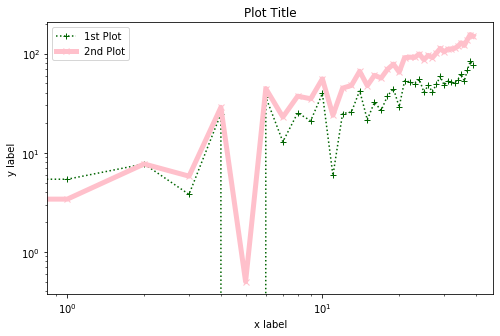
\includegraphics[width=0.7\textwidth]{figures/axis2}
	\caption{Example of log-scale plot.}
	\label{fig:axis2}
\end{figure}

\subsubsection{Date on Axis}\label{date-on-axis}

A special need, very common in finance, is to have dates on the \(x\)
axis. This can be done like shown in the next example and in Figure~\ref{fig:axis3}:

\begin{ipython}
import datetime as dt
import matplotlib.dates as mdates

dates = ['01/02/1991','01/03/1991','01/04/1991']
xd = [dt.datetime.strptime(d,'%m/%d/%Y').date() for d in dates]
yd = range(len(xd))
fig = plt.figure(figsize=(8,5))
plt.gca().xaxis.set_major_formatter(mdates.DateFormatter('%m/%d/%Y'))
plt.gca().xaxis.set_major_locator(mdates.DayLocator())
plt.plot(xd, yd)
plt.gcf().autofmt_xdate() # this makes a prettier formatting
plt.show()
\end{ipython}

\begin{figure}[h]
	\centering
	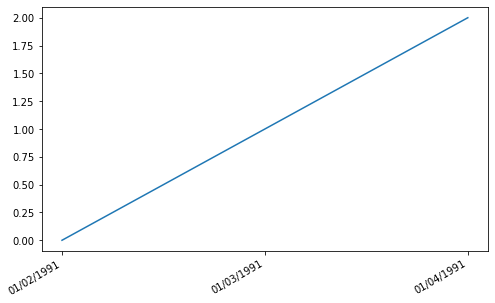
\includegraphics[width=0.6\textwidth]{figures/axis3}
	\caption{Plotting with dates on the $x$ axis.}
	\label{fig:axis3}
\end{figure}

\subsection{Subplots}
\label{subplots}

It may happen that we need to plot two or more plots side by side or in
a grid fashion.

The canvas can be then split into sub-canvases with the \texttt{subplot}
commands which takes in input the number of rows, columns and the index
of the current subplot. It returns the \emph{sub-canvas} object that can
be used to draw like previously shown.

There is one complication though, some of the commands change when
dealing with subplot: \texttt{xlabel} and \texttt{ylabel} for example
becomes \texttt{set\_xlabel} and \texttt{set\_ylabel}. Similarly for
\texttt{xlim} and \texttt{ylim}.

As an example imagine that we want to plot previous data side by
side on two canvases instead of together in the same (Fig.~\ref{fig:subplot})

\begin{ipython}
fig = plt.figure(figsize=(8,5))
sub1 = plt.subplot(1, 2, 1)
sub1.plot(x, y1, marker="+", linestyle=":", color="darkgreen", label="1st Plot")
sub1.set_xlabel("x label")
sub1.set_ylabel("y label")
sub1.legend()
sub2 = plt.subplot(1, 2, 2)
sub2.plot(x, y2, marker="x", linewidth=5, color="pink", label="2nd Plot")
sub2.set_xlabel("x label")
sub2.set_ylabel("y label")
sub2.legend()
plt.show()
\end{ipython}

\begin{figure} [htb]
	\centering
	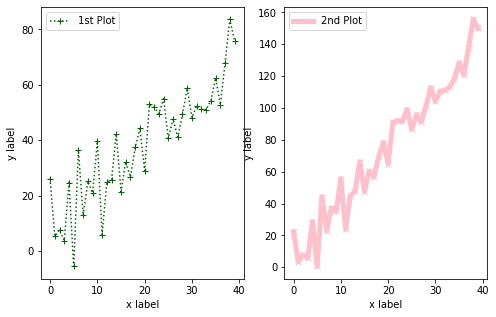
\includegraphics[width=0.65\textwidth]{figures/subplot}
	\caption{Example of subplots.}
	\label{fig:subplot}
\end{figure}

Subplots can also be arranged in another way like, see instead Figure~\ref{fig:subplot2}

\begin{ipython}
fig = plt.figure(figsize=(8,5))
sub1 = plt.subplot(2, 1, 1)
sub1.plot(x, y1, marker="+", linestyle=":", color="darkgreen", label="1st Plot")
sub1.set_xlabel("x label")
sub1.set_ylabel("y label")
sub1.legend()
sub2 = plt.subplot(2, 1, 2)
sub2.plot(x, y2, marker="x", linewidth=5, color="pink", label="2nd Plot")
sub2.set_xlabel("x label")
sub2.set_ylabel("y label")
sub2.legend()
plt.show()
\end{ipython}

%FIXME share the same axis xlabel plot 1 is covered
\begin{figure}[h]
	\centering
	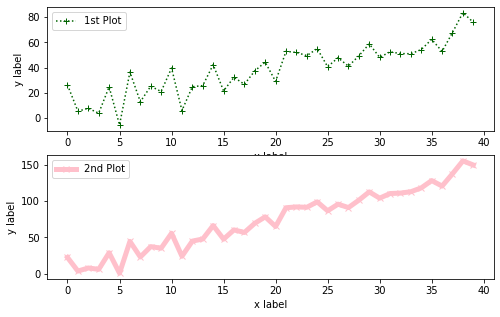
\includegraphics[width=0.65\textwidth]{figures/subplot2}
	\caption{Different arrangement of the two subplots.}
	\label{fig:subplot2}
\end{figure}

\subsection{Lines and Text}\label{lines-and-text}

To make plots more informative it can be useful to add text or lines on
a plot.

\subsubsection{Lines}\label{lines}

Lines can be drawn with \texttt{hlines} (for horizontal lines) and
\texttt{hvines} (for vertical lines). Both commands take in input the
\texttt{y}, \texttt{x\_min}, \texttt{x\_max} and \texttt{x}, \texttt{y\_min}, \texttt{y\_max}
respectively. Beware, coordinates are relative to the axis scale.

Other parameters allow to format the line in terms of color, style,
width\ldots. Look for example at Fig.~\ref{fig:lines}

\begin{ipython}
fig = plt.figure(figsize=(8,5))
plt.plot(x, y1, marker="+", linestyle=":", color="darkgreen", label="1st Plot")
plt.plot(x, y2, marker="x", linewidth=5, color="pink", label="2nd Plot")
plt.title("Plot Title")
plt.xlabel("x label")
plt.ylabel("y label")
plt.hlines(65, 0, 37.5, color='red', linestyle="-.", label='Critical Thr.')
plt.legend()
plt.show()
\end{ipython}

\begin{figure}[htb]
	\centering
	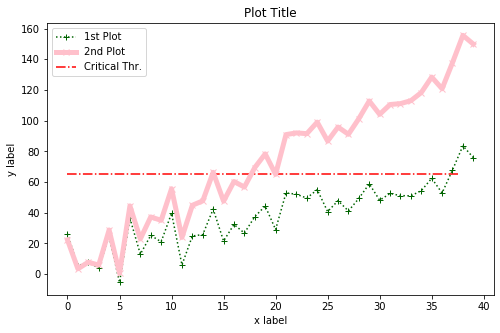
\includegraphics[width=0.7\textwidth]{figures/lines}
	\caption{Adding lines to our plots.}
	\label{fig:lines}
\end{figure}

Notice as the \(y\) value is 65 and \(x\) goes from 0 to 37.5 which
corresponds to each axis.

Analogously for a vertical line, except that we have to first specify
the \(x\) value and then the \(y\) range (Fig.~\ref{fig:lines2}).

\begin{ipython}
fig = plt.figure(figsize=(8,5))
plt.plot(x, y1, marker="+", linestyle=":", color="darkgreen", label="1st Plot")
plt.plot(x, y2, marker="x", linewidth=5, color="pink", label="2nd Plot")
plt.title("Plot Title")
plt.xlabel("x label")
plt.ylabel("y label")
plt.vlines(22, 0, 120, color='gray', label='Splitting Thr.')
plt.legend()
plt.show()
\end{ipython}

\begin{figure}[htb]
	\centering
	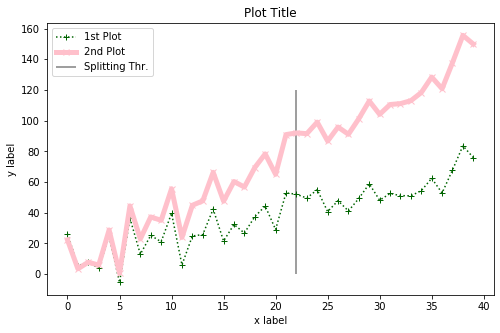
\includegraphics[width=0.7\textwidth]{figures/lines2}
	\caption{Vertical lines.}
	\label{fig:lines2}
\end{figure}

\subsubsection{Text}\label{text}

Like lines text can be added to the plot with the command \texttt{text}.
This function takes the \texttt{x} and \texttt{y} coordinates of starting point of
the text and the actual text string. Like before coordinates are
relative to the axis plot.

Other options can be used to format the text style, their meaning should
be straightforward:

\begin{itemize}
	\tightlist
	\item
	\texttt{backgroundcolor};
	\item
	\texttt{color};
	\item
	\texttt{fontfamily}: (FONTNAME, `serif', `sans-serif', `cursive', `fantasy', `monospace');
	\item
	\texttt{fontsize}; (size in points, `xx-small', `x-small', `small', `medium', `large', `x-large', `xx-large');
	\item
	\texttt{fontstyle}: (`normal', `italic', `oblique');
	\item
	\texttt{horizontalalignment}: (`center', `right', `left');
	\item
	\texttt{rotation}: takes the angle in degrees;
	\item
	\texttt{verticalalignment}: (`center', `top', `bottom', `baseline', `center\_baseline').
\end{itemize}

\begin{ipython}
fig = plt.figure(figsize=(8,5))
plt.plot(x, y1, marker="+", linestyle=":", color="darkgreen", label="1st Plot")
plt.plot(x, y2, marker="x", linewidth=5, color="pink", label="2nd Plot")
plt.title("Plot Title")
plt.xlabel("x label")
plt.ylabel("y label")
plt.vlines(22, 0, 120, color='gray')
plt.text(23, 5, "Splitting Thr.", rotation=90)
plt.hlines(65, 0, 37.5, color='red', linestyle="-.")
plt.text(25, 75, "Critical Thr.", backgroundcolor="red", color="white")
plt.legend()
plt.show()
\end{ipython}

\begin{figure}[htb]
	\centering
	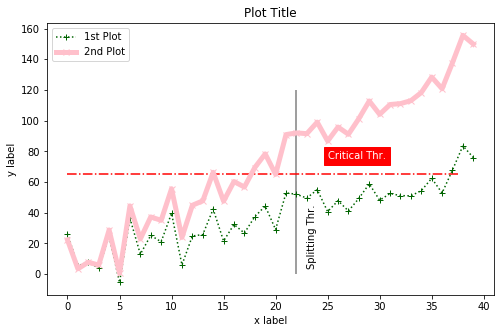
\includegraphics[width=0.7\textwidth]{figures/text}
	\caption{Adding also some text to our plot.}
	\label{fig:text}
\end{figure}

\subsection{Saving}\label{saving}

A plot can be saved into a file for later usage with \texttt{savefig} which takes in input the file name. The format of the file will be inferred from the file name extension (.jpg, .png, .gif\ldots)

\begin{ipython}
plt.savefig("myfigure.png")
\end{ipython}

%\subsection{Plot a graph given \(x\) and \(y\) values (scatter-plot)}\label{plot-a-graph-given-x-and-y-values}
%
%\begin{codebox}
%\begin{Verbatim}[commandchars=\\\{\}]
%\PY{k+kn}{from} \PY{n+nn}{matplotlib} \PY{k}{import} \PY{n}{pyplot} \PY{k}{as} \PY{n}{plt}
%
%\PY{n}{x} \PY{o}{=} \PY{p}{[}\PY{l+m+mi}{1}\PY{p}{,} \PY{l+m+mi}{2}\PY{p}{,} \PY{l+m+mi}{3}\PY{p}{]}
%\PY{n}{y} \PY{o}{=} \PY{p}{[}\PY{l+m+mf}{0.3}\PY{p}{,} \PY{l+m+mf}{0.4}\PY{p}{,} \PY{l+m+mf}{0.6}\PY{p}{]}
% 
%\PY{n}{plt}\PY{o}{.}\PY{n}{plot}\PY{p}{(}\PY{n}{x}\PY{p}{,} \PY{n}{y}\PY{p}{,} \PY{n}{marker}\PY{o}{=}\PY{l+s+s1}{\PYZsq{}}\PY{l+s+s1}{o}\PY{l+s+s1}{\PYZsq{}}\PY{p}{)} \PY{c+c1}{\PYZsh{} we are using circle markers}
%\PY{n}{plt}\PY{o}{.}\PY{n}{grid}\PY{p}{(}\PY{k+kc}{True}\PY{p}{)}               \PY{c+c1}{\PYZsh{} this line activate grid drawing}
%\PY{n}{plt}\PY{o}{.}\PY{n}{show}\PY{p}{(}\PY{p}{)}
%\end{Verbatim}
%\end{codebox}
%
%\begin{figure}[h]
%\centering
%  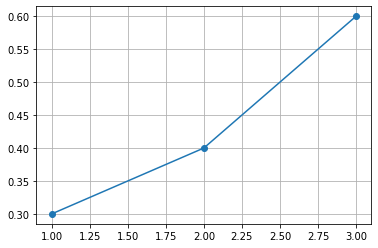
\includegraphics[width=0.6\textwidth]{figures/Untitled_43_0.png}
%\end{figure}
%%    { \hspace*{\fill} \\}
%    
%\begin{codebox}
%\begin{Verbatim}[commandchars=\\\{\}]
%\PY{c+c1}{\PYZsh{} if we want to plot specific points too}
%
%\PY{n}{x} \PY{o}{=} \PY{p}{[}\PY{l+m+mi}{1}\PY{p}{,} \PY{l+m+mi}{2}\PY{p}{,} \PY{l+m+mi}{3}\PY{p}{]}
%\PY{n}{y} \PY{o}{=} \PY{p}{[}\PY{l+m+mf}{0.3}\PY{p}{,} \PY{l+m+mf}{0.4}\PY{p}{,} \PY{l+m+mf}{0.6}\PY{p}{]}
% 
%\PY{n}{plt}\PY{o}{.}\PY{n}{plot}\PY{p}{(}\PY{n}{x}\PY{p}{,} \PY{n}{y}\PY{p}{,} \PY{n}{marker}\PY{o}{=}\PY{l+s+s1}{\PYZsq{}}\PY{l+s+s1}{x}\PY{l+s+s1}{\PYZsq{}}\PY{p}{)}
%\PY{n}{plt}\PY{o}{.}\PY{n}{plot}\PY{p}{(}\PY{l+m+mf}{2.5}\PY{p}{,} \PY{l+m+mf}{0.5}\PY{p}{,} \PY{n}{marker}\PY{o}{=}\PY{l+s+s1}{\PYZsq{}}\PY{l+s+s1}{X}\PY{l+s+s1}{\PYZsq{}}\PY{p}{,} \PY{n}{ms}\PY{o}{=}\PY{l+m+mi}{12}\PY{p}{,} \PY{n}{color}\PY{o}{=}\PY{l+s+s1}{\PYZsq{}}\PY{l+s+s1}{red}\PY{l+s+s1}{\PYZsq{}}\PY{p}{)}
%\PY{n}{plt}\PY{o}{.}\PY{n}{plot}\PY{p}{(}\PY{l+m+mf}{1.5}\PY{p}{,} \PY{l+m+mf}{0.35}\PY{p}{,} \PY{n}{marker}\PY{o}{=}\PY{l+s+s1}{\PYZsq{}}\PY{l+s+s1}{x}\PY{l+s+s1}{\PYZsq{}}\PY{p}{,} \PY{n}{ms}\PY{o}{=}\PY{l+m+mi}{12}\PY{p}{,} \PY{n}{color}\PY{o}{=}\PY{l+s+s1}{\PYZsq{}}\PY{l+s+s1}{red}\PY{l+s+s1}{\PYZsq{}}\PY{p}{)}
%\PY{n}{plt}\PY{o}{.}\PY{n}{grid}\PY{p}{(}\PY{k+kc}{True}\PY{p}{)}              
%\PY{n}{plt}\PY{o}{.}\PY{n}{show}\PY{p}{(}\PY{p}{)}
%\end{Verbatim}
%\end{codebox}
%
%\begin{figure}[h]
%\centering
%  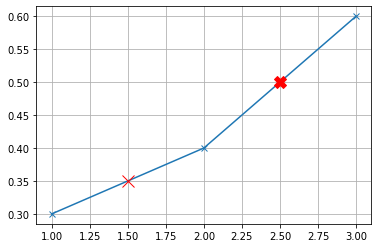
\includegraphics[width=0.6\textwidth]{figures/Untitled_44_0.png}
%\end{figure}
%%    { \hspace*{\fill} \\}
%    
%\subsubsection{What if \(x\) values are dates ?}
%
%\begin{codebox}
%\begin{Verbatim}[commandchars=\\\{\}]
%\PY{k+kn}{import} \PY{n+nn}{datetime}
%\PY{k+kn}{import} \PY{n+nn}{matplotlib}\PY{n+nn}{.}\PY{n+nn}{dates} \PY{k}{as} \PY{n+nn}{mdates}
%
%\PY{n}{x} \PY{o}{=} \PY{p}{[}\PY{n}{datetime}\PY{o}{.}\PY{n}{date}\PY{p}{(}\PY{l+m+mi}{2020}\PY{p}{,} \PY{l+m+mi}{7}\PY{p}{,} \PY{l+m+mi}{20}\PY{p}{)}\PY{p}{,}  \PY{n}{datetime}\PY{o}{.}\PY{n}{date}\PY{p}{(}\PY{l+m+mi}{2020}\PY{p}{,} \PY{l+m+mi}{7}\PY{p}{,} \PY{l+m+mi}{30}\PY{p}{)}\PY{p}{,} 
%     \PY{n}{datetime}\PY{o}{.}\PY{n}{date}\PY{p}{(}\PY{l+m+mi}{2020}\PY{p}{,} \PY{l+m+mi}{8}\PY{p}{,} \PY{l+m+mi}{10}\PY{p}{)}\PY{p}{,}  \PY{n}{datetime}\PY{o}{.}\PY{n}{date}\PY{p}{(}\PY{l+m+mi}{2020}\PY{p}{,} \PY{l+m+mi}{8}\PY{p}{,} \PY{l+m+mi}{20}\PY{p}{)}\PY{p}{]}
%     
%\PY{n}{y} \PY{o}{=} \PY{p}{[}\PY{l+m+mi}{10}\PY{p}{,} \PY{l+m+mi}{20}\PY{p}{,} \PY{l+m+mi}{34}\PY{p}{,} \PY{l+m+mi}{45}\PY{p}{]}
%\PY{n}{plt}\PY{o}{.}\PY{n}{plot}\PY{p}{(}\PY{n}{x}\PY{p}{,} \PY{n}{y}\PY{p}{,} \PY{n}{marker}\PY{o}{=}\PY{l+s+s1}{\PYZsq{}}\PY{l+s+s1}{o}\PY{l+s+s1}{\PYZsq{}}\PY{p}{)}
%\PY{c+c1}{\PYZsh{} this line tells matplotlib we have dates on x axis}
%\PY{n}{plt}\PY{o}{.}\PY{n}{gca}\PY{p}{(}\PY{p}{)}\PY{o}{.}\PY{n}{xaxis}\PY{o}{.}\PY{n}{set\PYZus{}major\PYZus{}formatter}\PY{p}{(}\PY{n}{mdates}\PY{o}{.}\PY{n}{DateFormatter}\PY{p}{(}\PY{l+s+s1}{\PYZsq{}}\PY{l+s+s1}{\PYZpc{}}\PY{l+s+s1}{Y\PYZhy{}}\PY{l+s+s1}{\PYZpc{}}\PY{l+s+s1}{m\PYZhy{}}\PY{l+s+si}{\PYZpc{}d}\PY{l+s+s1}{\PYZsq{}}\PY{p}{)}\PY{p}{)}
%\PY{c+c1}{\PYZsh{} this one instead rotate labels to avoid superimposition}
%\PY{n}{plt}\PY{o}{.}\PY{n}{xticks}\PY{p}{(}\PY{n}{rotation}\PY{o}{=}\PY{l+m+mi}{45}\PY{p}{)}
%\PY{n}{plt}\PY{o}{.}\PY{n}{grid}\PY{p}{(}\PY{k+kc}{True}\PY{p}{)}
%\PY{n}{plt}\PY{o}{.}\PY{n}{show}\PY{p}{(}\PY{p}{)}
%\end{Verbatim}
%\end{codebox}
%
%\begin{figure}[h]
%\centering
%  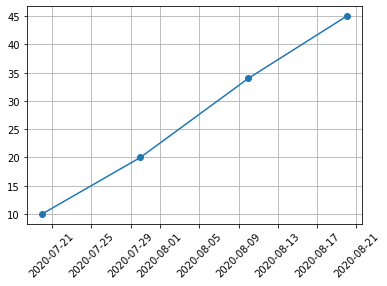
\includegraphics[width=0.6\textwidth]{figures/Untitled_46_0.png}
%\end{figure}
%%    { \hspace*{\fill} \\}
%    
%\subsection{Plotting an Histogram}\label{plotting-an-histogram}
%
%\begin{codebox}
%\begin{Verbatim}[commandchars=\\\{\}]
%\PY{k+kn}{import} \PY{n+nn}{random} 
%\PY{n}{numbers} \PY{o}{=} \PY{p}{[}\PY{p}{]}
%\PY{k}{for} \PY{n}{\PYZus{}} \PY{o+ow}{in} \PY{n+nb}{range}\PY{p}{(}\PY{l+m+mi}{1000}\PY{p}{)}\PY{p}{:}
%  \PY{n}{numbers}\PY{o}{.}\PY{n}{append}\PY{p}{(}\PY{n}{random}\PY{o}{.}\PY{n}{randint}\PY{p}{(}\PY{l+m+mi}{1}\PY{p}{,} \PY{l+m+mi}{10}\PY{p}{)}\PY{p}{)}
%
%\PY{k+kn}{from} \PY{n+nn}{matplotlib} \PY{k}{import} \PY{n}{pyplot} \PY{k}{as} \PY{n}{plt}
%
%\PY{c+c1}{\PYZsh{} Here we define the binning}
%\PY{c+c1}{\PYZsh{} 6 is the number of bins, going from 0 to 10}
%\PY{n}{plt}\PY{o}{.}\PY{n}{hist}\PY{p}{(}\PY{n}{numbers}\PY{p}{,} \PY{l+m+mi}{10}\PY{p}{,} \PY{n+nb}{range}\PY{o}{=}\PY{p}{[}\PY{l+m+mi}{0}\PY{p}{,} \PY{l+m+mi}{11}\PY{p}{]}\PY{p}{)} 
%\PY{n}{plt}\PY{o}{.}\PY{n}{show}\PY{p}{(}\PY{p}{)}
%\end{Verbatim}
%\end{codebox}
%
%\begin{figure}[h]
%\centering
%  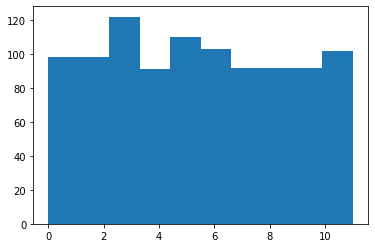
\includegraphics[width=0.55\textwidth]{figures/Untitled_48_0.png}
%\end{figure}
% %   { \hspace*{\fill} \\}
%    
%\subsubsection{Plotting a Function}\label{plotting-a-function}
%
%In this case let's try to make the plot prettier adding labels, legend\ldots{}
%All the commands apply also to the previous examples.
%
%\begin{codebox}
%\begin{Verbatim}[commandchars=\\\{\}]
%\PY{k+kn}{import} \PY{n+nn}{numpy} \PY{k}{as} \PY{n+nn}{np}
%\PY{k+kn}{import} \PY{n+nn}{matplotlib}\PY{n+nn}{.}\PY{n+nn}{pyplot} \PY{k}{as} \PY{n+nn}{plt}
%\PY{k+kn}{from} \PY{n+nn}{scipy}\PY{n+nn}{.}\PY{n+nn}{stats} \PY{k}{import} \PY{n}{norm}
%
%\PY{c+c1}{\PYZsh{} define the functions to plot}
%\PY{c+c1}{\PYZsh{} a gaussian with mean=0  and sigma=1}
%\PY{c+c1}{\PYZsh{} in scipy module this is called norm}
%\PY{n}{mu}\PY{o}{=}\PY{l+m+mi}{0}
%\PY{n}{sigma} \PY{o}{=} \PY{l+m+mi}{1}
%\PY{n}{x} \PY{o}{=} \PY{n}{np}\PY{o}{.}\PY{n}{arange}\PY{p}{(}\PY{o}{\PYZhy{}}\PY{l+m+mi}{10}\PY{p}{,} \PY{o}{\PYZhy{}}\PY{l+m+mf}{1.645}\PY{p}{,} \PY{l+m+mf}{0.001}\PY{p}{)}
%\PY{n}{x\PYZus{}all} \PY{o}{=} \PY{n}{np}\PY{o}{.}\PY{n}{arange}\PY{p}{(}\PY{o}{\PYZhy{}}\PY{l+m+mi}{4}\PY{p}{,} \PY{l+m+mi}{4}\PY{p}{,} \PY{l+m+mf}{0.001}\PY{p}{)}
%\PY{n}{y} \PY{o}{=} \PY{n}{norm}\PY{o}{.}\PY{n}{pdf}\PY{p}{(}\PY{n}{x}\PY{p}{,} \PY{l+m+mi}{0}\PY{p}{,} \PY{l+m+mi}{1}\PY{p}{)}
%\PY{n}{y\PYZus{}all} \PY{o}{=} \PY{n}{norm}\PY{o}{.}\PY{n}{pdf}\PY{p}{(}\PY{n}{x\PYZus{}all}\PY{p}{,} \PY{l+m+mi}{0}\PY{p}{,} \PY{l+m+mi}{1}\PY{p}{)}
%
%\PY{c+c1}{\PYZsh{} draw the gaussian}
%\PY{n}{plt}\PY{o}{.}\PY{n}{plot}\PY{p}{(}\PY{n}{x\PYZus{}all}\PY{p}{,} \PY{n}{y\PYZus{}all}\PY{p}{,} \PY{n}{label}\PY{o}{=}\PY{l+s+s1}{\PYZsq{}}\PY{l+s+s1}{Gaussian}\PY{l+s+s1}{\PYZsq{}}\PY{p}{)}
%
%\PY{c+c1}{\PYZsh{} fill with different alpha using x\PYZus{}all and y\PYZus{}all as limits}
%\PY{c+c1}{\PYZsh{} alpha set the transparency level: 0 trasparent, 1 solid}
%\PY{n}{plt}\PY{o}{.}\PY{n}{fill\PYZus{}between}\PY{p}{(}\PY{n}{x\PYZus{}all}\PY{p}{,} \PY{n}{y\PYZus{}all}\PY{p}{,} \PY{l+m+mi}{0}\PY{p}{,} \PY{n}{alpha}\PY{o}{=}\PY{l+m+mf}{0.1}\PY{p}{,} \PY{n}{color}\PY{o}{=}\PY{l+s+s1}{\PYZsq{}}\PY{l+s+s1}{blue}\PY{l+s+s1}{\PYZsq{}}\PY{p}{,} \PY{n}{label}\PY{o}{=}\PY{l+s+s2}{\PYZdq{}}\PY{l+s+s2}{Gaussian CDF}\PY{l+s+s2}{\PYZdq{}}\PY{p}{)}
%
%\PY{c+c1}{\PYZsh{} fill with color red using x and y as limits}
%\PY{c+c1}{\PYZsh{} label associate text to the object for the legend}
%\PY{n}{plt}\PY{o}{.}\PY{n}{fill\PYZus{}between}\PY{p}{(}\PY{n}{x}\PY{p}{,} \PY{n}{y}\PY{p}{,} \PY{l+m+mi}{0}\PY{p}{,} \PY{n}{alpha}\PY{o}{=}\PY{l+m+mi}{1}\PY{p}{,} \PY{n}{color}\PY{o}{=}\PY{l+s+s1}{\PYZsq{}}\PY{l+s+s1}{red}\PY{l+s+s1}{\PYZsq{}}\PY{p}{,} \PY{n}{label}\PY{o}{=}\PY{l+s+s2}{\PYZdq{}}\PY{l+s+s2}{5}\PY{l+s+s2}{\PYZpc{}}\PY{l+s+s2}{ tail}\PY{l+s+s2}{\PYZdq{}}\PY{p}{)}
%
%\PY{c+c1}{\PYZsh{} set x axis limits}
%\PY{n}{plt}\PY{o}{.}\PY{n}{xlim}\PY{p}{(}\PY{p}{[}\PY{o}{\PYZhy{}}\PY{l+m+mi}{4}\PY{p}{,} \PY{l+m+mi}{4}\PY{p}{]}\PY{p}{)}
%
%\PY{c+c1}{\PYZsh{} add a label for X axis}
%\PY{n}{plt}\PY{o}{.}\PY{n}{xlabel}\PY{p}{(}\PY{l+s+s2}{\PYZdq{}}\PY{l+s+s2}{Changes of value}\PY{l+s+s2}{\PYZdq{}}\PY{p}{)}
%
%\PY{c+c1}{\PYZsh{} add a label to y axis}
%\PY{n}{plt}\PY{o}{.}\PY{n}{ylabel}\PY{p}{(}\PY{l+s+s2}{\PYZdq{}}\PY{l+s+s2}{Gaussian values}\PY{l+s+s2}{\PYZdq{}}\PY{p}{)}
%
%\PY{c+c1}{\PYZsh{} add histogram title}
%\PY{n}{plt}\PY{o}{.}\PY{n}{title}\PY{p}{(}\PY{l+s+s2}{\PYZdq{}}\PY{l+s+s2}{Distribution of changes of value}\PY{l+s+s2}{\PYZdq{}}\PY{p}{)}
%
%\PY{c+c1}{\PYZsh{} draw a vertical line at x=\PYZhy{}1.645}
%\PY{c+c1}{\PYZsh{} y limits are in percent w.r.t. to y axis length}
%\PY{n}{plt}\PY{o}{.}\PY{n}{axvline}\PY{p}{(}\PY{n}{x}\PY{o}{=}\PY{o}{\PYZhy{}}\PY{l+m+mf}{1.645}\PY{p}{,} \PY{n}{ymin}\PY{o}{=}\PY{l+m+mf}{0.1}\PY{p}{,} \PY{n}{ymax}\PY{o}{=}\PY{l+m+mi}{1}\PY{p}{,} \PY{n}{linestyle}\PY{o}{=}\PY{l+s+s1}{\PYZsq{}}\PY{l+s+s1}{:}\PY{l+s+s1}{\PYZsq{}}\PY{p}{,} \PY{n}{linewidth}\PY{o}{=}\PY{l+m+mi}{1}\PY{p}{,} \PY{n}{color} \PY{o}{=} \PY{l+s+s1}{\PYZsq{}}\PY{l+s+s1}{red}\PY{l+s+s1}{\PYZsq{}}\PY{p}{)}
%
%\PY{c+c1}{\PYZsh{} write some text to explain the line}
%\PY{n}{plt}\PY{o}{.}\PY{n}{text}\PY{p}{(}\PY{o}{\PYZhy{}}\PY{l+m+mf}{1.9}\PY{p}{,} \PY{o}{.}\PY{l+m+mi}{12}\PY{p}{,} \PY{l+s+s1}{\PYZsq{}}\PY{l+s+s1}{95}\PY{l+s+s1}{\PYZpc{}}\PY{l+s+s1}{ percentile (VaR loss)}\PY{l+s+s1}{\PYZsq{}}\PY{p}{,}\PY{n}{fontsize}\PY{o}{=}\PY{l+m+mi}{10}\PY{p}{,} \PY{n}{rotation}\PY{o}{=}\PY{l+m+mi}{90}\PY{p}{,} 
%                                    \PY{n}{color}\PY{o}{=}\PY{l+s+s1}{\PYZsq{}}\PY{l+s+s1}{red}\PY{l+s+s1}{\PYZsq{}}\PY{p}{)}
%
%\PY{n}{plt}\PY{o}{.}\PY{n}{legend}\PY{p}{(}\PY{p}{)}
%\PY{n}{plt}\PY{o}{.}\PY{n}{show}\PY{p}{(}\PY{p}{)}
%\end{Verbatim}
%\end{codebox}
%
%\begin{figure}[htp]
%\centering
%  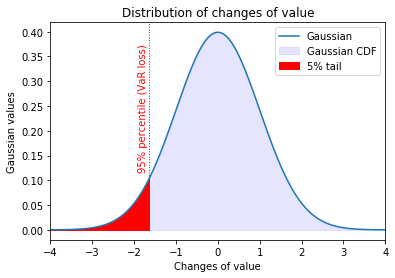
\includegraphics[width=0.55\textwidth]{figures/Untitled_50_0.png}
%\end{figure}
%%    { \hspace*{\fill} \\}
%    \clearpage
%If you are particularly satisfied by your work you can save the graph to a file:
%
%\begin{codebox}
%\begin{Verbatim}[commandchars=\\\{\}]
%\PY{n}{plt}\PY{o}{.}\PY{n}{savefig}\PY{p}{(}\PY{l+s+s1}{\PYZsq{}}\PY{l+s+s1}{normal\PYZus{}curve.png}\PY{l+s+s1}{\PYZsq{}}\PY{p}{)}
%
%<Figure size 432x288 with 0 Axes>
%
%\end{Verbatim}
%\end{codebox}

\section{Exercises}
\begin{question}
Using \texttt{pandas} import data stored in \href{https://drive.google.com/file/d/1Uu9lQorvzM-1xwRKPNszaSqlCYAiY-gr/view?usp=sharing}{\texttt{stock\_market.xlsx}}. With the resulting dataframe determine:
\begin{itemize}
\item remove duplicates and missing data (how many rows are left ?);
\item stocks with positive variation;
\item the first five stocks with the lowest price.
\end{itemize}
\end{question}

\begin{solution}
First load the excel file into a dataframe and look at data structure.
\end{solution}

\begin{ipython}
import pandas as pd

df = pd.read_excel("stock_market.xlsx")
print (len(df))
df.head()

51

  Symbol                      Name   Price  Change  Change%  Volume (M)  \
0     GE  General Electric Company    6.07   -0.19  -0.0304     142.732
1    NOK         Nokia Corporation    4.78    0.33   0.0742     117.960
2      F        Ford Motor Company    6.61   -0.13  -0.0193     115.394
3   PINS           Pinterest, Inc.   34.29    9.10   0.3613     111.864
4   AAPL                Apple Inc.  425.04   40.28   0.1047      93.574

   Avg Volume (M)  Market Cap (B)
0         102.268          53.132
1          31.296          27.083
2          87.719          26.288
3          15.550          20.110
4          35.035        1821.000
\end{ipython}
        
As usual if we are not sure that our data is \emph{clean} we should check for duplicates and NaN and take care of them. The \texttt{duplicated} method returns the status of each row (duplicate or not, True or False). If we would like just to see the duplicated entries we could combine the \texttt{duplicated} method with the selection syntax like this:

\begin{ipython}
df[df.duplicated() == True]

   Symbol         Name  Price  Change  Change%  Volume (M)  Avg Volume (M)  \
40    RUN  Sunrun Inc.  36.69    0.02   0.0005      20.113           3.604

    Market Cap (B)
40           4.489
\end{ipython}
        
So it looks like we have just one duplicate and we can remove it:

\begin{ipython}
print ("Before duplicates removal: {}".format(len(df)))
df = df.drop_duplicates()
print ("After duplicates removal: {}".format(len(df)))

Before duplicates removal: 50
After duplicates removal: 50
\end{ipython}

Then we need to take care of the NaN, again if we want to check the rows with NaN we can select (here the syntax is a little bit more complicated since we need to use \texttt{any} to look for Nan in every column):

\begin{ipython}
df[df.isna().any(axis=1)]

   Symbol                                 Name  Price  Change  Change%  \
23   NCLH  Norwegian Cruise Line Holdings Ltd.  13.64   -0.53  -0.0374
47    NBL                   Noble Energy, Inc.    NaN   -0.23  -0.0225

    Volume (M)  Avg Volume (M)  Market Cap (B)
23      28.402          64.895             NaN
47      18.462          13.535           4.795
\end{ipython}
        
Since we don't want to artificially modify our sample we just drop rows with NaN:

\begin{ipython}
print ("Before NaN removal: {}".format(len(df)))
df = df.dropna()
print ("After NaN removal: {}".format(len(df)))

Before NaN removal: 51
After NaN removal: 49
\end{ipython}

The second point asks to determine the companies with a daily positive variation. Clearly we have to apply to the dataframe a selection on the "Change" (or "change\%") column requiring positive values.

\begin{ipython}
pos_var = df[df.loc[:, "Change"] > 0]
print (len(pos_var))
pos_var.head() # just printing the first 5 rows

16

  Symbol                         Name   Price  Change  Change%  Volume (M)  \
1    NOK            Nokia Corporation    4.78    0.33   0.0742     117.960
3   PINS              Pinterest, Inc.   34.29    9.10   0.3613     111.864
4   AAPL                   Apple Inc.  425.04   40.28   0.1047      93.574
6    BAC  Bank of America Corporation   24.88    0.04   0.0016      62.039
8     FB               Facebook, Inc.  253.67   19.17   0.0817      53.030

   Avg Volume (M)  Market Cap (B)
1          31.296          27.083
3          15.550          20.110
4          35.035        1821.000
6          72.793         215.562
8          24.521         723.726
\end{ipython}
        
So in origin we had 48 stocks and just 16 have a positive variation of its price.

The last question requires to print the first 5 stocks with the lowest prices. In this case it is enough to sort by price the dataframe (ascending) and then just select the first 5 entries.

\begin{ipython}
highest_price = df.sort_values(by=['Price'], ascending=True)[:5]
highest_price

   Symbol                      Name  Price  Change  Change%  Volume (M)  \
25   ABEV               Ambev S. A.   2.68   -0.16  -0.0563      26.136
32    BBD      Banco Bradesco S. A.   4.22   -0.32  -0.0705      22.129
1     NOK         Nokia Corporation   4.78    0.33   0.0742     117.960
15    OPK         OPKO Health, Inc.   5.15   -0.76  -0.1286      35.762
33    MRO  Marathon Oil Corporation   5.49   -0.02  -0.0036      21.249

    Avg Volume (M)  Market Cap (B)
25          36.654          41.999
32          22.046          36.739
1           31.296          27.083
15          17.792           3.450
33          34.098           4.339
\end{ipython}


\begin{question}
Given the following discount factors plot the resulting discount curve,
possibly adding axis labels and legend.
\end{question}

\begin{ipython}
dfs = [1.0, 1.0014907894567657, 1.0031038833235129, 1.0047764800189012,
       1.0065986105304596, 1.014496095021891, 1.022687560553011,
       1.0303585751965112, 1.0369440287181253, 1.0422287558021188,
       1.0461834022163963, 1.0489228953047331, 1.0505725627906783, 
       1.0513323539753632, 1.0513777790851995, 1.0508768750534248,
       1.049935905228433, 1.0486741093761602, 1.047175413484517,
       1.0455115431993336, 1.0437147446170034, 1.0418294960952215,
       1.0398823957504923, 1.0378979499878478, 1.0358789099539805,
       1.0338409767365169, 1.031791178324756, 1.0297378455884902,
       1.0276772747965244, 1.0256154380560942, 1.0235543974485939,
       1.0214974135391857, 1.0194401540150835, 1.0173862951028778]

pillars = [datetime.date(2020, 8, 3), datetime.date(2020, 11, 3),
		   datetime.date(2021, 2, 3), datetime.date(2021, 5, 3),
		   datetime.date(2021, 8, 3), datetime.date(2022, 8, 3),
		   datetime.date(2023, 8, 3), datetime.date(2024, 8, 3),
		   datetime.date(2025, 8, 3), datetime.date(2026, 8, 3),
		   datetime.date(2027, 8, 3), datetime.date(2028, 8, 3),
		   datetime.date(2029, 8, 3), datetime.date(2030, 8, 3),
		   datetime.date(2031, 8, 3), datetime.date(2032, 8, 3),
		   datetime.date(2033, 8, 3), datetime.date(2034, 8, 3),
		   datetime.date(2035, 8, 3), datetime.date(2036, 8, 3),
		   datetime.date(2037, 8, 3), datetime.date(2038, 8, 3),
		   datetime.date(2039, 8, 3), datetime.date(2040, 8, 3),
		   datetime.date(2041, 8, 3), datetime.date(2042, 8, 3),
		   datetime.date(2043, 8, 3), datetime.date(2044, 8, 3),
		   datetime.date(2045, 8, 3), datetime.date(2046, 8, 3),
		   datetime.date(2047, 8, 3), datetime.date(2048, 8, 3),
           datetime.date(2049, 8, 3), datetime.date(2050, 8, 3)]
\end{ipython}

\begin{solution}
\end{solution}

\begin{ipython}
import datetime
from matplotlib import pyplot as plt
import matplotlib.dates as mdates

dfs = [1.0, 1.0014907894567657, 1.0031038833235129, 1.0047764800189012, ...]
pillars = [datetime.date(2020, 8, 3), datetime.date(2020, 11, 3), ...]

plt.plot(pillars, dfs, marker="o", label="EUR6M d.f.")

plt.gca().xaxis.set_major_formatter(mdates.DateFormatter('%Y-%m-%d'))
# this one instead rotate labels to avoid superimposition
plt.xticks(rotation=45)
plt.xlabel("Pillar dates")
plt.ylabel("Discount Factors")
plt.grid(True)
plt.legend()
plt.show()
\end{ipython}

\begin{figure}[htb]
\begin{center}
  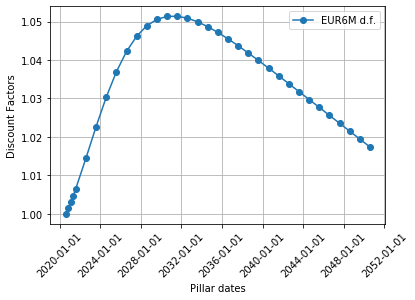
\includegraphics[width=0.7\linewidth]{figures/ex5.5.png}
\end{center}
\end{figure}





\begin{thebibliography}{9}
  %  %\bibitem{survey2019} StackOverflow \emph{The TEXbook}, Addison-Wesley, Reading,Massachusetts, second edition, 1984,
\bibitem{pandas} \href{https://pandas.pydata.org/docs/}{\emph{Pandas Official Documentation}} [Online]
\bibitem{matplotlib} \href{https://matplotlib.org}{\emph{Matplotlib Official Documentation}} [Online]
\bibitem{bib:quandl} \href{https://docs.quandl.com/}{\emph{Quandl Documentation}} [Online]
\bibitem{bib:yfinance} \href{https://github.com/ranaroussi/yfinance}{\emph{YFinance Documentation}} [Online]
\bibitem{bib:ffn} \href{https://pmorissette.github.io/ffn/}{\emph{Financial Functions for Python}} [Online]
\end{thebibliography}
